% =====================================================================
%  Rotation-equivariant direction finding for non-terrestrial networks
%  Draft letter (arXiv), IEEEtran conference style
%  Compile: pdflatex main; pdflatex main
% =====================================================================
\documentclass[conference]{IEEEtran}
\IEEEoverridecommandlockouts

\usepackage{cite}
\usepackage{amsmath,amssymb,amsfonts}
\usepackage{graphicx}
\usepackage{xcolor}
\usepackage{booktabs}
\usepackage{url}
\usepackage{tikz}
\usetikzlibrary{arrows.meta,calc,positioning,fit,backgrounds,decorations.pathreplacing}
\usepackage{pgfplots}
\pgfplotsset{compat=1.18}
\usepackage[hidelinks]{hyperref}

% ---- shared colors for figures ----
\definecolor{cMLP}{HTML}{6B7280}
\definecolor{cTrans}{HTML}{1F5C8B}
\definecolor{cEquiv}{HTML}{C8881C}
\definecolor{cBart}{HTML}{2E7D5B}
\definecolor{cFail}{HTML}{B23A3A}

\newcommand{\E}[1]{\mathbf{e}_{#1}}

\begin{document}

\title{Geometric Equivariance as an Inductive Bias for\\
Orientation-Robust Direction Finding in\\
Non-Terrestrial Networks}

\author{\IEEEauthorblockN{Do Phuc Hao}
\IEEEauthorblockA{Faculty of Information Technology\\
Da Nang Architecture University, Da Nang, Vietnam\\
haodp@dau.edu.vn}}

\maketitle

\begin{abstract}
Non-terrestrial networks (NTN) and space-air-ground integrated networks (SAGIN)
place antenna arrays on satellites and aerial platforms whose orientation varies
continuously, so a direction-of-arrival (DOA) estimator must remain accurate at
array orientations never seen during training. We study how a known geometric
symmetry of this task, the rotation of the array, should be exploited, and we use
geometric algebra (GA) as the language in which that symmetry is explicit. On a
controlled uniform circular array (UCA) probe, azimuth rotation reduces exactly to
a cyclic shift of the sensor index, the simplest instance of the geometric
equivariance that GA and Clifford networks generalize. We compare three options:
ignore the symmetry, augment for it with random cyclic shifts, or build it into a
$C_M$-equivariant circular-convolution network, all against a classical Bartlett
beamformer and over five seeds. Built-in equivariance and augmentation both reach
the classical accuracy at large training sets, but equivariance is more data
efficient at small sets, markedly more stable across seeds, with augmented
non-equivariant models, the Transformer in particular, sometimes failing to
converge, and it uses the fewest parameters. A classical beamformer matches all
learned models on the clean single-source task, but on a two-source single-snapshot
task both learned models resolve separations of about half the classical beamwidth,
and the equivariant model alone resolves the hardest case, with an order of magnitude
fewer parameters than the augmented baseline. We frame the result as a controlled
account of how a geometric symmetry should enter a learned NTN array model, and as a
proof of concept for the machine-learning pillar of a broader program that uses GA as
a unifying substrate across the quantum and learning layers of NTN and SAGIN. Code is
released for reproducibility.
\end{abstract}

\begin{IEEEkeywords}
Geometric algebra, equivariant learning, direction of arrival, non-terrestrial
networks, SAGIN, inductive bias.
\end{IEEEkeywords}

% ---- Main flow / overview figure (spans both columns) ----
\begin{figure*}[t]
\centering
\resizebox{\textwidth}{!}{%
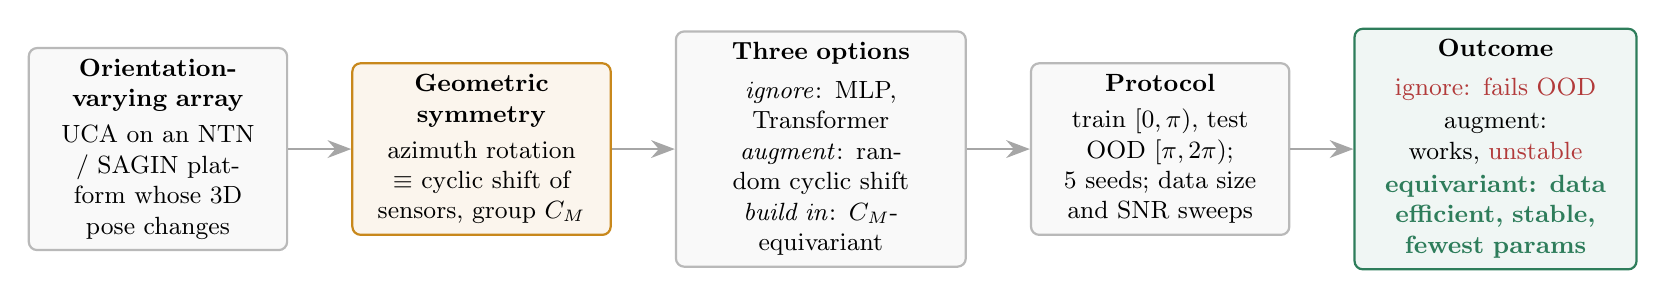
\begin{tikzpicture}[font=\small, >=Stealth, node distance=8mm,
  stage/.style={rounded corners=3pt, draw=gray!55, line width=0.8pt, align=center,
                fill=gray!5, minimum height=2.0cm, text width=3.0cm, inner sep=4pt},
  ar/.style={-{Stealth[length=3mm]}, line width=1pt, gray!70}]

  % Stage A: array with rotation icon
  \node[stage] (a)
     {\textbf{Orientation-varying array}\\[2pt]
      UCA on an NTN / SAGIN platform whose 3D pose changes};
  % small UCA glyph inside-ish (above the label)
  \begin{scope}[shift={($(a.north)+(0,0.05)$)}]
  \end{scope}

  % Stage B: symmetry
  \node[stage, right=of a, draw=cEquiv, fill=cEquiv!8] (b)
     {\textbf{Geometric symmetry}\\[2pt]
      azimuth rotation $\equiv$ cyclic shift of sensors, group $C_M$};

  % Stage C: three ways to handle the symmetry
  \node[stage, right=of b, text width=3.4cm] (c)
     {\textbf{Three options}\\[3pt]
      \textit{ignore}: MLP, Transformer\\
      \textit{augment}: random cyclic shift\\
      \textit{build in}: $C_M$-equivariant};

  % Stage D: protocol
  \node[stage, right=of c] (d)
     {\textbf{Protocol}\\[2pt]
      train $[0,\pi)$, test OOD $[\pi,2\pi)$;\\ 5 seeds; data size and SNR sweeps};

  % Stage E: outcome
  \node[stage, right=of d, draw=cBart, fill=cBart!7, text width=3.3cm] (e)
     {\textbf{Outcome}\\[3pt]
      \textcolor{cFail}{ignore: fails OOD}\\[1pt]
      augment: works, \textcolor{cFail}{unstable}\\[1pt]
      \textcolor{cBart}{\textbf{equivariant: data efficient, stable, fewest params}}};

  \draw[ar] (a)--(b); \draw[ar] (b)--(c); \draw[ar] (c)--(d); \draw[ar] (d)--(e);
\end{tikzpicture}}
\caption{Main flow of the study. The array orientation varies, so the task carries
a known geometric symmetry: rotating the source azimuth equals a cyclic shift of
the sensors (group $C_M$). We compare ignoring the symmetry, augmenting for it, and
building it in. Augmentation closes most of the gap at large data, but built-in
equivariance is more data efficient, more stable, and lighter.}
\label{fig:flow}
\end{figure*}

% =====================================================================
\section{Introduction}
% =====================================================================
Mobile network coverage is moving into a genuinely three-dimensional regime.
Non-terrestrial networks (NTN) integrate low-earth-orbit satellites, high-altitude
platform stations, and unmanned aerial vehicles into 5G and 6G, and space-air-ground
integrated networks (SAGIN) fuse the space, air, and ground tiers into a single
system \cite{sagin2018}. A defining feature of this regime is that the antenna
array is carried by a platform whose three-dimensional orientation changes
continuously. A model that learns a physical-layer function such as
direction-of-arrival (DOA) estimation must therefore stay accurate at array
orientations, and consequently at incident angles, that were never present in the
training set.

Standard data-driven estimators do not provide this guarantee for free. A network
that memorizes a mapping from array snapshots to angles within the training
support has no reason to behave correctly outside that support. The principled
remedy is to bake the relevant symmetry into the model, so that rotating the array
rotates the prediction in lockstep. This is the equivariance principle that
underlies geometric deep learning, and geometric algebra (GA), the real Clifford
algebra of Euclidean space, is a natural language for it: rotations are rotors,
data are multivectors, and the symmetry group acts uniformly on every quantity.

This letter asks a deliberately narrow and verifiable question, then places it in a
wider context. The question is how a known geometric symmetry of the task should
enter a learned estimator, comparing three options: ignore it, augment for it, or
build it in. The wider context is a research program in which GA serves as a common
substrate spanning two pillars of NTN and SAGIN: the quantum pillar, where a qubit
is a rotor and quantum gates are real multivector operations, and the
machine-learning pillar, where Clifford and equivariant networks process geometric
signals. The present experiment is a proof of concept for the second pillar only.
Figure~\ref{fig:flow} summarizes the study.

Our contributions are as follows.
\begin{itemize}
\item We formulate orientation-robust DOA on a uniform circular array (UCA) as a
group-equivariance problem and show that azimuth rotation reduces exactly to a
cyclic shift of the sensor index, the discrete rotation group $C_M$.
\item We compare, at matched parameter budget and over five seeds, three ways of
handling this symmetry, namely a symmetry-agnostic MLP and Transformer, the same
models trained with cyclic-shift augmentation, and a $C_M$-equivariant
circular-convolution network, against a classical Bartlett beamformer, across
training-set size and SNR.
\item We find that augmentation and built-in equivariance both attain the classical
accuracy at large data, but equivariance is more data efficient, substantially more
stable across seeds, and lighter, and we discuss honestly what this does and does
not establish.
\item We show, on a two-source single-snapshot task, that the learned models resolve
sources about twice as close as the classical beamformer, the equivariant one most
parameter-efficiently and alone at the hardest separation, which is where learning
exceeds rather than inherits the classical behavior.
\end{itemize}

% =====================================================================
\section{Background and Positioning}
% =====================================================================
\subsection{Geometric algebra as a shared language}
Geometric algebra builds on the geometric product $ab = a\cdot b + a\wedge b$,
which combines the scalar inner product and the bivector outer product. Rotations
in any dimension are represented by rotors $R=\exp(-\mathbf{B}\,\theta/2)$ acting
through the two-sided map $v\mapsto R\,v\,\tilde{R}$. Two branches of this
formalism are mature. In wireless and radar signal processing, GA has long been
used for conformal-array pattern analysis, distortionless co-polarization
beamforming, and DOA estimation on vector-sensor arrays, with reported reductions
in computational and memory cost relative to long-vector and Euler-angle
formulations \cite{zou2011,meng2017,wang2021}. In quantum theory, the Pauli
matrices are the basis vectors of $\mathrm{Cl}(3,0)$, a qubit is a rotor, and the
multiparticle spacetime algebra expresses qubit states and unitary gates, together
with universality, as real multivector operations \cite{haveldoran2000,doran1996,cafaro2011,cafaro2024}.

\subsection{Equivariant learning, classical and quantum}
On the learning side, Clifford neural layers embed data as multivectors and respect
the geometric product \cite{clifford2022,cliffordlayers}, and the geometric algebra
transformer uses a projective Clifford algebra as its internal representation to be
equivariant to the Euclidean group $\mathrm{E}(3)$ \cite{gatr2023}. The same
symmetry idea appears on the quantum side: group-invariant and equivariant quantum
neural networks respect the symmetry of the data and thereby mitigate trainability
and generalization problems such as barren plateaus
\cite{larocca2022,nguyen2024}. Equivariance is thus a bridge that appears on both
the classical and the quantum side, yet no prior work, to our knowledge, uses GA
as a single language across both layers for NTN or SAGIN. We do not close that gap
here; we validate the classical half of it on a concrete network task and report
the result without overclaiming. Our equivariant model is the discrete rotation
instance of this principle, which heavier Clifford and $\mathrm{E}(3)$-equivariant
architectures generalize.

\subsection{Learning-based DOA and the gap}
Learned DOA estimation was established by grid-based classifiers and regressors on
linear arrays, from the multitask autoencoder of Liu \emph{et al.} \cite{liu2018}
to the per-subregion spectrum regressor DeepMUSIC \cite{elbir2020}, and later made
gridless and extended to complex-valued and Transformer architectures
\cite{wu2022,tan2023,guo2024}. Robustness to array imperfections, including mutual
coupling and gain and phase errors, has been pursued by training the network over
sampled perturbations, as in SDOA-Net \cite{sdoanet2024}. Two patterns recur across this literature. First, the array is
almost always linear, so the rotational structure of a circular aperture is not
used. Second, robustness and generalization are obtained by training over
variations, which is augmentation, rather than by an architectural symmetry
constraint. The only genuinely equivariant DOA networks we are aware of are
acoustic, such as the icosahedral CNN that approximates $\mathrm{SO}(3)$ for
sound-source localization \cite{diazguerra2023}, not RF antenna arrays. To our
knowledge, no RF DOA network builds cyclic-group $C_M$ equivariance on a uniform
circular array, none studies generalization to unseen array orientations or angular
sectors, none reports a controlled equivariance-versus-augmentation comparison, and
none is motivated by non-terrestrial geometries. This letter addresses that gap.

% =====================================================================
\section{Signal Model and Equivariant Network}
% =====================================================================
\subsection{Array model and the rotation symmetry}
Consider a UCA of $M$ sensors in the $xy$-plane, with sensor $i$ at angular
position $\gamma_i = 2\pi i/M$. For a single narrowband far-field source at azimuth
$\phi$ and fixed elevation, the response of sensor $i$ is
\begin{equation}
a_i(\phi) = \exp\!\big(\,j\,\kappa\,\cos(\phi-\gamma_i)\,\big),
\qquad \kappa = \tfrac{2\pi}{\lambda}\,r,
\label{eq:steer}
\end{equation}
with array radius $r$. The observation is $x_i = a_i(\phi) + n_i$ with complex
white Gaussian noise $n_i$ at a prescribed signal-to-noise ratio (SNR). The key
structural fact follows from \eqref{eq:steer}:
\begin{equation}
a_i\!\big(\phi + \tfrac{2\pi}{M}\big)
= \exp\!\big(j\kappa\cos(\phi-\gamma_{i-1})\big)
= a_{i-1}(\phi).
\label{eq:shift}
\end{equation}
Rotating the source azimuth (equivalently, rotating the array about its axis) by
one inter-sensor angle is exactly a cyclic shift of the sensor index. Azimuth
rotation is therefore the cyclic group $C_M$ acting on the sensor axis. Figure
\ref{fig:uca} illustrates this.

\begin{figure}[t]
\centering
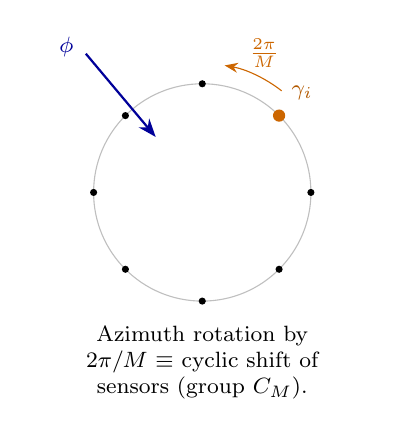
\begin{tikzpicture}[scale=0.92, >=Stealth, font=\footnotesize]
  \draw[gray!50] (0,0) circle (1.5);
  \foreach \k in {0,...,7}{
    \fill[black] (\k*45:1.5) circle (1.4pt);
  }
  \fill[orange!80!black] (45:1.5) circle (2.4pt);
  \node[orange!70!black] at (45:1.95) {$\gamma_i$};
  % incoming wave direction
  \draw[->, blue!60!black, thick] (130:2.5) -- (130:1.0);
  \node[blue!60!black] at (133:2.75) {$\phi$};
  % rotation hint
  \draw[->, orange!80!black] (52:1.78) arc (52:80:1.78);
  \node[orange!80!black] at (66:2.1) {$\tfrac{2\pi}{M}$};
  \node[align=center, text width=4.2cm] at (0,-2.35)
    {Azimuth rotation by $2\pi/M$ $\equiv$ cyclic shift of sensors (group $C_M$).};
\end{tikzpicture}
\caption{Uniform circular array. By \eqref{eq:shift}, rotating the source azimuth
by one inter-sensor angle permutes the sensor responses cyclically, so a circular
convolution over the sensors is equivariant to array rotation.}
\label{fig:uca}
\end{figure}

\subsection{Models}
All learned models map the two-channel real signal $x\in\mathbb{R}^{2\times M}$
(real and imaginary parts) to a two-vector that is normalized to a predicted unit
direction $(\cos\hat\phi,\sin\hat\phi)$, and are trained with the squared error on
that unit direction.

\textbf{MLP.} The signal is flattened and passed through fully connected layers.
This model has no rotation inductive bias.

\textbf{Transformer.} Each sensor is a token carrying its real and imaginary parts
plus a fixed cyclic positional encoding $(\cos\gamma_i,\sin\gamma_i)$, followed by
self-attention and average pooling. Attention is permutation equivariant and the
positional encoding injects geometry, but the model is not exactly
$C_M$-equivariant.

\textbf{EquivCircConv (equivariant).} The signal is processed by circular
convolution layers (\texttt{Conv1d} with circular padding), which are
cyclic-shift equivariant. The final layer outputs an $M$-bin angular spectrum, and
a soft-argmax over the bin directions $(\cos\gamma_b,\sin\gamma_b)$ produces the
prediction:
\begin{equation}
\hat{v} = \sum_{b=1}^{M} \mathrm{softmax}(\ell)_b
          \,(\cos\gamma_b,\sin\gamma_b),
\end{equation}
where $\ell$ are the spectrum logits. A cyclic shift of the input shifts $\ell$ by
one bin and hence rotates $\hat v$ by $2\pi/M$, so the matched filter learned on
$[0,\pi)$ transfers to $[\pi,2\pi)$. This is the $C_M$-equivariant realization of
the GA equivariance principle.

\textbf{Cyclic-shift augmentation.} The MLP and the Transformer are also trained
with augmentation, our fair non-equivariant baseline. By \eqref{eq:shift}, rolling
the sensor axis by $s$ steps equals an azimuth rotation by $2\pi s/M$, so during
training we roll each input by a random $s$ and rotate its target by the same
angle. This exposes a symmetry-agnostic model to the full rotation group without
changing its architecture.

\textbf{Bartlett (classical reference).} A non-learned conventional beamformer
scans a fine azimuth grid and returns the peak of $|a(\phi_b)^{\mathsf H}x|^2$. It
is rotation equivariant by physics and needs no training.

% =====================================================================
\section{Experimental Setup}
% =====================================================================
We use $M=16$ sensors and $\kappa=\pi$ (radius $r=0.5\lambda$). Training azimuths
are drawn uniformly from $[0,\pi)$; we evaluate on a fixed held-out
in-distribution (ID) set with azimuths in $[0,\pi)$ and a fixed out-of-distribution
(OOD) set with azimuths in $[\pi,2\pi)$, each of size $2000$, with single-snapshot
observations. Every configuration is run over five seeds, and we report the mean
and standard deviation. Models are trained for $80$ epochs with Adam, a cosine
schedule, and batch size $128$. We run two studies: a data-efficiency study that
sweeps the training size over $\{200,500,1000,2000,5000\}$ at $10$\,dB SNR, and an
SNR study that sweeps the SNR over $\{0,5,10,15,20\}$\,dB at a fixed training size
of $1000$. The metric is the mean absolute circular azimuth error in degrees.
Parameter counts are $31{,}362$ (MLP), $17{,}346$ (Transformer), and $10{,}817$
(equivariant); augmentation does not change them, so the equivariant model is the
smallest.

% =====================================================================
\section{Results}
% =====================================================================
\subsection{Single source: equivariance versus augmentation}
Table \ref{tab:main} summarizes OOD and ID errors, and Figs.~\ref{fig:eff} and
\ref{fig:snr} show the data-efficiency and SNR studies. Four observations stand out.

\begin{table}[t]
\caption{OOD azimuth error (deg, mean $\pm$ std over 5 seeds) at the smallest and
largest training sizes, ID error at $N{=}5000$, and parameter count. ID is
$[0,\pi)$, OOD is $[\pi,2\pi)$.}
\label{tab:main}
\centering
\small
\setlength{\tabcolsep}{4pt}
\begin{tabular}{@{}lccccc@{}}
\toprule
Model & OOD $N{=}200$ & OOD $N{=}5000$ & ID $N{=}5000$ & Params \\
\midrule
MLP             & $130.0\!\pm\!1.6$ & $126.8\!\pm\!2.5$ & $1.20$ & 31.4k \\
\;+aug          & $2.90\!\pm\!0.44$ & $1.23\!\pm\!0.01$ & $1.21$ & 31.4k \\
Transformer     & $115.8\!\pm\!10$  & $117.3\!\pm\!17$  & $1.37$ & 17.3k \\
\;+aug          & $90.7\!\pm\!34$   & $10.8\!\pm\!18$   & $27.9$ & 17.3k \\
\textbf{Equivariant} & $\mathbf{1.88\!\pm\!0.62}$ & $\mathbf{1.21\!\pm\!0.01}$ & $\mathbf{1.19}$ & \textbf{10.8k} \\
\midrule
Bartlett        & $1.19$ & $1.19$ & $1.19$ & 0 \\
\bottomrule
\end{tabular}
\end{table}

\begin{figure}[t]
\centering
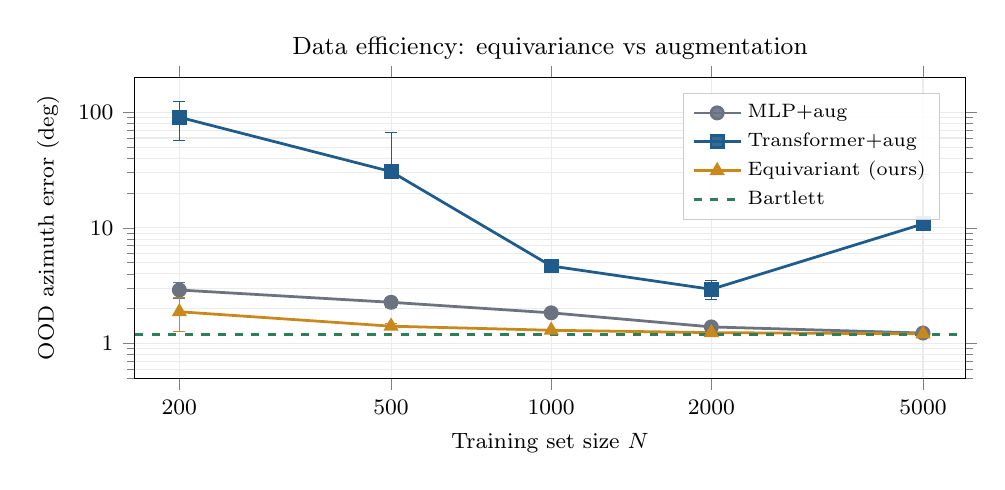
\begin{tikzpicture}
\begin{semilogxaxis}[
  width=\columnwidth, height=5.4cm,
  xlabel={Training set size $N$}, ylabel={OOD azimuth error (deg)},
  xmin=165, xmax=6000, ymode=log, ymin=0.5, ymax=200,
  xtick={200,500,1000,2000,5000}, xticklabels={200,500,1000,2000,5000},
  log ticks with fixed point, tick align=outside,
  grid=both, grid style={gray!16},
  legend cell align=left,
  legend style={font=\scriptsize, at={(0.97,0.95)}, anchor=north east, draw=gray!40,
                fill=white, fill opacity=0.9, text opacity=1},
  every axis plot/.append style={line width=1pt, mark size=2.2pt},
  title style={font=\small, yshift=-1mm},
  title={Data efficiency: equivariance vs augmentation},
  label style={font=\footnotesize}, tick label style={font=\footnotesize},
]
\addplot[cMLP, mark=*, error bars/.cd, y dir=both, y explicit]
  coordinates {(200,2.90)+-(0,0.44)(500,2.27)+-(0,0.22)(1000,1.84)+-(0,0.02)(2000,1.39)+-(0,0.04)(5000,1.23)+-(0,0.01)};
\addplot[cTrans, mark=square*, error bars/.cd, y dir=both, y explicit]
  coordinates {(200,90.70)+-(0,33.98)(500,30.70)+-(0,35.84)(1000,4.68)+-(0,0.53)(2000,2.94)+-(0,0.54)(5000,10.82)+-(0,18.38)};
\addplot[cEquiv, mark=triangle*, error bars/.cd, y dir=both, y explicit]
  coordinates {(200,1.88)+-(0,0.62)(500,1.41)+-(0,0.09)(1000,1.30)+-(0,0.02)(2000,1.24)+-(0,0.01)(5000,1.21)+-(0,0.01)};
\addplot[cBart, dashed, line width=1pt] coordinates {(165,1.19)(6000,1.19)};
\legend{MLP+aug, Transformer+aug, Equivariant (ours), Bartlett}
\end{semilogxaxis}
\end{tikzpicture}
\caption{Data efficiency (log scale). Augmentation and equivariance both approach
the classical beamformer at large $N$, but the equivariant model is lower at small
$N$ and far more stable; the augmented Transformer is erratic (large error bars).
The symmetry-agnostic MLP and Transformer, omitted for clarity, stay above
$110^\circ$ at every $N$ (Table~\ref{tab:main}).}
\label{fig:eff}
\end{figure}

\begin{figure}[t]
\centering
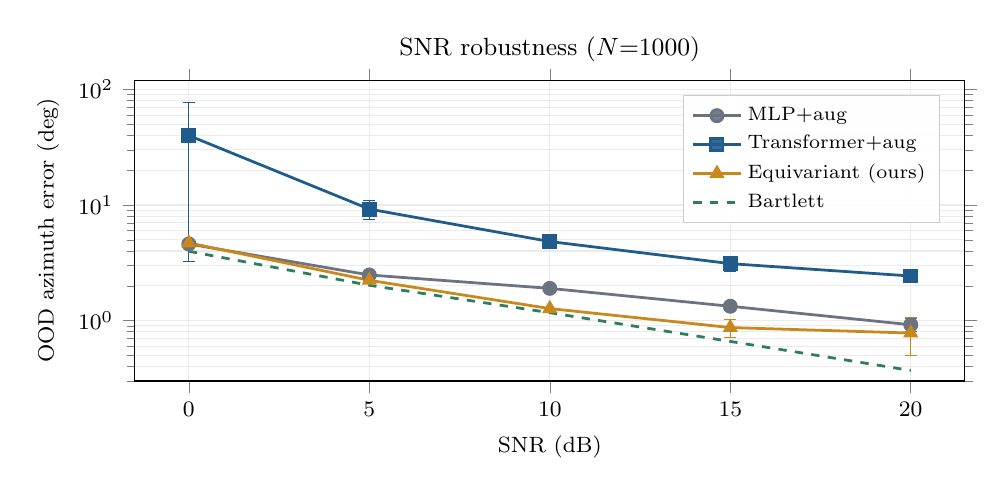
\begin{tikzpicture}
\begin{axis}[
  width=\columnwidth, height=5.4cm,
  xlabel={SNR (dB)}, ylabel={OOD azimuth error (deg)},
  xmin=-1.5, xmax=21.5, ymode=log, ymin=0.3, ymax=120,
  xtick={0,5,10,15,20}, tick align=outside,
  grid=both, grid style={gray!16},
  legend cell align=left,
  legend style={font=\scriptsize, at={(0.97,0.95)}, anchor=north east, draw=gray!40,
                fill=white, fill opacity=0.9, text opacity=1},
  every axis plot/.append style={line width=1pt, mark size=2.2pt},
  title style={font=\small, yshift=-1mm},
  title={SNR robustness ($N{=}1000$)},
  label style={font=\footnotesize}, tick label style={font=\footnotesize},
]
\addplot[cMLP, mark=*, error bars/.cd, y dir=both, y explicit]
  coordinates {(0,4.60)+-(0,0.07)(5,2.48)+-(0,0.12)(10,1.90)+-(0,0.16)(15,1.33)+-(0,0.10)(20,0.92)+-(0,0.12)};
\addplot[cTrans, mark=square*, error bars/.cd, y dir=both, y explicit]
  coordinates {(0,39.96)+-(0,36.72)(5,9.22)+-(0,1.66)(10,4.83)+-(0,0.61)(15,3.11)+-(0,0.47)(20,2.43)+-(0,0.15)};
\addplot[cEquiv, mark=triangle*, error bars/.cd, y dir=both, y explicit]
  coordinates {(0,4.70)+-(0,0.11)(5,2.23)+-(0,0.03)(10,1.27)+-(0,0.01)(15,0.87)+-(0,0.15)(20,0.78)+-(0,0.28)};
\addplot[cBart, dashed, line width=1pt, mark=none]
  coordinates {(0,3.98)(5,2.02)(10,1.17)(15,0.66)(20,0.37)};
\legend{MLP+aug, Transformer+aug, Equivariant (ours), Bartlett}
\end{axis}
\end{tikzpicture}
\caption{SNR robustness at $N{=}1000$ (log scale). The equivariant model tracks the
classical beamformer across SNR and is the best learned model; the augmented
baselines lag, the Transformer markedly so and with high variance at low SNR.}
\label{fig:snr}
\end{figure}

First, ignoring the symmetry fails. The symmetry-agnostic MLP and Transformer stay
above $110^\circ$ on OOD azimuths at every training size and SNR (Table
\ref{tab:main}), confirming that a model fit on a restricted azimuth range does not
extrapolate to unseen orientations.

Second, augmentation largely closes the gap, which is the honest comparison a
strong baseline demands. The augmented MLP falls from $2.90^\circ$ at $N{=}200$ to
$1.23^\circ$ at $N{=}5000$, essentially reaching the classical reference. Any claim
that equivariance is needed merely to generalize across orientations would be
overstated.

Third, equivariance still wins on the axes that matter for deployment. It is more
data efficient, reaching $1.88^\circ$ at $N{=}200$ against the augmented MLP's
$2.90^\circ$, and it is far more stable: its standard deviation stays near
$0.01^\circ$ to $0.6^\circ$, whereas the augmented Transformer is erratic, with
standard deviations above $30^\circ$ and a seed that fails to converge (its ID error
at $N{=}5000$ is $27.9^\circ$). It also uses one third of the MLP parameters and
needs no augmentation schedule. Across SNR (Fig.~\ref{fig:snr}) the equivariant
model tracks the beamformer and stays ahead of the augmented baselines.

Fourth, the classical Bartlett beamformer matches or beats every learned model on
this clean single-source task, at zero parameters. On this probe the learned models
inherit, rather than exceed, the classical behavior; the next subsection shows where
they exceed it.

\subsection{Two sources: beating the classical resolution limit}
The single-source probe is robust enough that learning adds nothing over the
beamformer. We therefore turn to the setting where classical beamforming is known to
fail, namely resolving two closely spaced sources. We place two equal-power sources
with a random relative phase at azimuths $\phi_c\pm\delta/2$, observe a single
snapshot, and declare a separation $\delta$ resolved when both sources are estimated
within $\delta/2$. Here the array radius is larger ($\kappa{=}8$, about half-wavelength
element spacing), giving a usable beamwidth. The equivariant model is extended to a
super-resolution form: it correlates the snapshot with the fine-grid steering
dictionary, which is the beamformer response and shifts cyclically under rotation, so
it stays $C_M$-equivariant, then circular convolutions deconvolve this response into
sharp peaks, trained with a peak-weighted loss. The augmented MLP uses the same front
end with fully connected layers.

Figure \ref{fig:res} reports the probability of resolution against separation, on OOD
azimuths and over three seeds. The classical beamformer needs about $30^\circ$ for
reliable resolution and resolves only $46\%$ of $15^\circ$ pairs. Both learned models
resolve almost perfectly from $15^\circ$, roughly half the classical limit, which is
the sense in which learning here exceeds classical beamforming. The two learned
models differ at the hardest separations and in size. At $12^\circ$ the equivariant
model resolves $67\%$ of pairs against $10\%$ for the augmented MLP and the
beamformer, although with high variance at this edge of resolvability, and it does so
with $34.6$k parameters against the augmented MLP's $295.8$k, an order of magnitude
fewer. Its in-distribution and out-of-distribution curves coincide, so the
resolution transfers across orientations.

\begin{figure}[t]
\centering
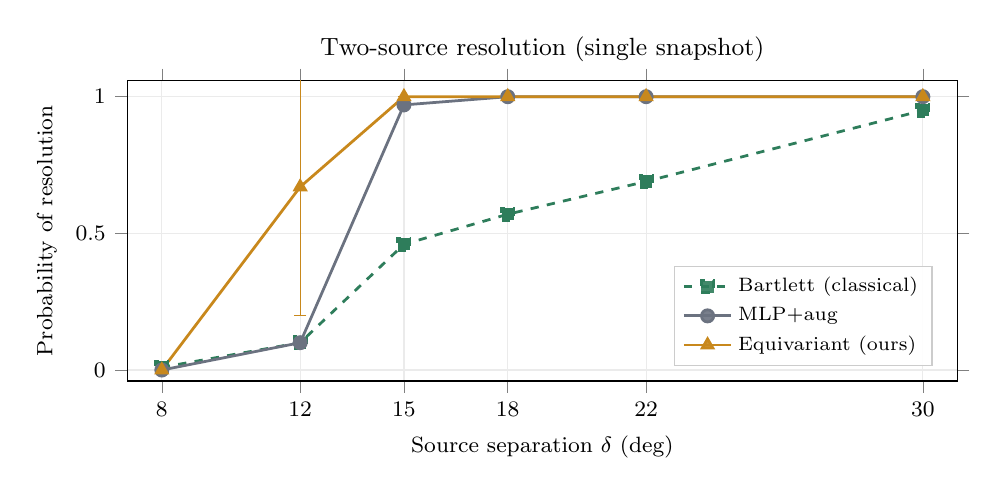
\begin{tikzpicture}
\begin{axis}[
  width=\columnwidth, height=5.4cm,
  xlabel={Source separation $\delta$ (deg)}, ylabel={Probability of resolution},
  xmin=7, xmax=31, ymin=-0.04, ymax=1.06,
  xtick={8,12,15,18,22,30}, tick align=outside,
  grid=both, grid style={gray!16},
  legend cell align=left,
  legend style={font=\scriptsize, at={(0.97,0.05)}, anchor=south east, draw=gray!40,
                fill=white, fill opacity=0.9, text opacity=1},
  every axis plot/.append style={line width=1pt, mark size=2.2pt},
  title style={font=\small, yshift=-1mm}, title={Two-source resolution (single snapshot)},
  label style={font=\footnotesize}, tick label style={font=\footnotesize},
]
\addplot[cBart, dashed, mark=square*]
  coordinates {(8,0.01)(12,0.10)(15,0.46)(18,0.57)(22,0.69)(30,0.95)};
\addplot[cMLP, mark=*, error bars/.cd, y dir=both, y explicit]
  coordinates {(8,0.0)+-(0,0.0)(12,0.10)+-(0,0.01)(15,0.97)+-(0,0.01)(18,1.0)+-(0,0.0)(22,1.0)+-(0,0.0)(30,1.0)+-(0,0.0)};
\addplot[cEquiv, mark=triangle*, error bars/.cd, y dir=both, y explicit]
  coordinates {(8,0.0)+-(0,0.0)(12,0.67)+-(0,0.47)(15,1.0)+-(0,0.0)(18,1.0)+-(0,0.0)(22,1.0)+-(0,0.0)(30,1.0)+-(0,0.0)};
\legend{Bartlett (classical), MLP+aug, Equivariant (ours)}
\end{axis}
\end{tikzpicture}
\caption{Two-source resolution probability versus separation, on OOD azimuths over
three seeds. Both learned models resolve from about $15^\circ$, half the classical
beamwidth; the equivariant model alone shows partial resolution at $12^\circ$, with
an order of magnitude fewer parameters. Its ID and OOD curves coincide.}
\label{fig:res}
\end{figure}

% =====================================================================
\section{Discussion}
% =====================================================================
\textbf{What this establishes.} When a task carries a known geometric symmetry,
both augmentation and built-in equivariance can exploit it, but they are not
equivalent. Augmentation reaches the same accuracy only with enough data and, on a
non-equivariant architecture, can be unstable to the point of non-convergence.
Built-in equivariance gives the same generalization more cheaply, more reliably,
and with fewer parameters. The right reading is therefore not equivariance versus
failure, but equivariance versus augmentation, where equivariance wins on data
efficiency and stability rather than on asymptotic accuracy. This is the behavior
the geometric learning literature predicts, here made concrete on an NTN-relevant
array task.

\textbf{Scope and limits.} On the clean single-source task a classical beamformer
already generalizes perfectly, so there the learned models inherit, rather than
exceed, the classical behavior, and we claim no advantage on raw in-distribution
accuracy. The two-source result is where learning exceeds classical, but it remains
controlled: a single snapshot, equal-power narrowband sources, and a planar circular
array. Multiple snapshots would admit a subspace baseline such as MUSIC, which a
fair study should include, and the equivariant advantage over augmentation in the
two-source case is confined to the hardest separation and to parameter count. We do
not validate the quantum pillar of the broader program here.

\textbf{Robustness to mutual coupling.} On a UCA the mutual-coupling matrix is
circulant and commutes with the cyclic shift, so coupling preserves the $C_M$
symmetry. The equivariant model is therefore correctly specified under coupling:
its OOD error stays near $1.2^\circ$ for reciprocal circulant coupling up to a
nearest-neighbour magnitude of $0.4$, matching the coupling-aware classical
beamformer. Prior robust DOA networks reach coupling robustness by training over
sampled perturbations \cite{liu2018,sdoanet2024}, the augmentation route we find
less stable; here the same robustness follows from the architecture. We note that
reciprocal coupling does not bias single-source DOA, so this regime is a robustness
check rather than a setting where learning beats classical; multi-source resolution
is the natural place to probe the latter.

\textbf{Toward a unified GA program for NTN and SAGIN.} The same equivariance that
helps here on the classical side has a quantum counterpart in group-equivariant
quantum neural networks, and GA expresses both with one set of operators. A
unified treatment that spans the quantum and the learning layers for NTN and
SAGIN, together with grounding in standardized non-terrestrial channel models such
as 3GPP TR 38.811, is the natural next step. Extending the probe to the conformal
arrays and full $\mathrm{SO}(3)$ orientations of real platforms, using Clifford and
$\mathrm{E}(3)$-equivariant layers, would test whether the present advantage
persists beyond the cyclic case.

% =====================================================================
\section{Conclusion}
% =====================================================================
We studied, on a controlled UCA direction-finding task motivated by non-terrestrial
networks, how a known array-rotation symmetry should enter a learned estimator.
Over five seeds and across training size and SNR, cyclic-shift augmentation and a
$C_M$-equivariant circular-convolution network both reach the classical accuracy at
large data, but the equivariant model is more data efficient, far more stable, and
uses the fewest parameters, while a classical beamformer matches all learned models
on this clean task. On a two-source single-snapshot task the learned models resolve
sources about twice as close as the beamformer, the equivariant one most cheaply and
alone at the hardest separation, which is where learning exceeds classical. We frame
this as a controlled account of how a geometric symmetry should be exploited, and as
a proof of concept for the machine-learning pillar of a broader vision in which
geometric algebra is a single language for both the quantum and the learning layers
of NTN and SAGIN.

% =====================================================================
\section*{Reproducibility}
The data generators, the models, the cyclic-shift augmentation, and the evaluation
for both the single-source and two-source studies are released as self-contained
Python scripts at \url{https://github.com/haodpsut/spl-paper}; all numbers in this
letter are produced by one run over fixed seeds.

\begin{thebibliography}{00}
\bibitem{sagin2018} J. Liu \emph{et al.}, ``Space-air-ground integrated network: A survey,'' \emph{IEEE Commun. Surveys Tuts.}, vol. 20, no. 4, pp. 2714--2741, 2018.
\bibitem{liu2018} Z.-M. Liu, C. Zhang, and P. S. Yu, ``Direction-of-arrival estimation based on deep neural networks with robustness to array imperfections,'' \emph{IEEE Trans. Antennas Propag.}, vol. 66, no. 12, pp. 7315--7327, 2018.
\bibitem{elbir2020} A. M. Elbir, ``DeepMUSIC: Multiple signal classification via deep learning,'' \emph{IEEE Sensors Lett.}, vol. 4, no. 4, 2020.
\bibitem{wu2022} X. Wu, X. Yang, X. Jia, and F. Tian, ``A gridless DOA estimation method based on convolutional neural network with Toeplitz prior,'' \emph{IEEE Signal Process. Lett.}, vol. 29, pp. 1247--1251, 2022.
\bibitem{tan2023} Z.-W. Tan, Y. Liu, A. W. H. Khong, and A. H. T. Nguyen, ``Gridless DOA estimation using complex-valued convolutional neural network with phasor normalization,'' \emph{IEEE Signal Process. Lett.}, vol. 30, pp. 813--817, 2023.
\bibitem{guo2024} Y. Guo, Z. Zhang, and Y. Huang, ``Dual class token vision transformer for direction of arrival estimation in low SNR,'' \emph{IEEE Signal Process. Lett.}, vol. 31, pp. 76--80, 2024.
\bibitem{sdoanet2024} P. Chen, Z. Chen, L. Liu, Y. Chen, and X. Wang, ``SDOA-Net: An efficient deep-learning-based DOA estimation network for imperfect array,'' \emph{IEEE Trans. Instrum. Meas.}, vol. 73, 2024, arXiv:2203.10231.
\bibitem{diazguerra2023} D. Diaz-Guerra, A. Miguel, and J. R. Beltran, ``Direction of arrival estimation with microphone arrays using $\mathrm{SO}(3)$-equivariant icosahedral CNNs,'' \emph{IEEE/ACM Trans. Audio, Speech, Lang. Process.}, vol. 31, 2023.
\bibitem{zou2011} Q. Zou, J. Lasenby, and Z. He, ``Beamforming with distortionless co-polarisation for conformal arrays based on geometric algebra,'' \emph{IET Radar, Sonar Navig.}, 2011.
\bibitem{meng2017} T. Meng, M. Wu, and N. Yuan, ``DOA estimation for conformal vector-sensor array using geometric algebra,'' \emph{EURASIP J. Adv. Signal Process.}, art. 64, 2017.
\bibitem{wang2021} M. Wang \emph{et al.}, ``Geometric algebra-based ESPRIT algorithm for DOA estimation,'' \emph{Sensors}, vol. 21, no. 17, art. 5933, 2021.
\bibitem{haveldoran2000} T. F. Havel and C. J. L. Doran, ``Geometric algebra in quantum information processing,'' \emph{AMS Contemp. Math.}, 2000, arXiv:quant-ph/0004031.
\bibitem{doran1996} C. Doran, A. Lasenby, S. Gull, S. Somaroo, and A. Challinor, ``Spacetime algebra and electron physics,'' \emph{Adv. Imaging Electron Phys.}, vol. 95, pp. 271--386, 1996.
\bibitem{cafaro2011} C. Cafaro and S. Mancini, ``A geometric algebra perspective on quantum computational gates and universality,'' \emph{Adv. Appl. Clifford Algebras}, vol. 21, pp. 493--519, 2011.
\bibitem{cafaro2024} C. Cafaro, N. Bahreyni, and L. Rossetti, ``From entanglement to universality: A multiparticle spacetime algebra approach revisited,'' \emph{Symmetry}, vol. 16, no. 6, art. 734, 2024.
\bibitem{clifford2022} J. Brandstetter, R. van den Berg, M. Welling, and J. K. Gupta, ``Clifford neural layers for PDE modeling,'' in \emph{Proc. ICLR}, 2023, arXiv:2209.04934.
\bibitem{cliffordlayers} Microsoft, ``CliffordLayers,'' github.com/microsoft/cliffordlayers, 2022.
\bibitem{gatr2023} J. Brehmer, P. de Haan, S. Behrends, and T. Cohen, ``Geometric algebra transformer,'' in \emph{Proc. NeurIPS}, 2023, arXiv:2305.18415.
\bibitem{larocca2022} M. Larocca \emph{et al.}, ``Group-invariant quantum machine learning,'' \emph{PRX Quantum}, vol. 3, art. 030341, 2022.
\bibitem{nguyen2024} Q. T. Nguyen \emph{et al.}, ``Theory for equivariant quantum neural networks,'' \emph{PRX Quantum}, vol. 5, art. 020328, 2024.
\end{thebibliography}

\end{document}